\chapter{Intensity Extraction, Fourier Maps and Charge-flipping}\label{Chap:intextraction}

In this chapter I will talk about how reflection intensities are estimated, including two intensity fitting methods, Pawley and Le Bail fits and then finally things that you can do in GSAS-II using the extracted intensities. 

\section{Rietveld's Intensity Extraction Method}

One long-standing problem back in the 1960's, when Hugo was busy developing Rietveld refinement, was how to come up with an estimate for the structure factors, $|F_{obs, hkl}|$, from a powder diffraction pattern. The problem being how to apportion out the intensity from overlapped reflections. This could be done for peaks that are not completely overlapped by use of deconvolution, but that was hard and slow back in those days and still did not solve the problem of how to apportion intensities for reflections that are exactly or very nearly overlapped. In any case, armed with estimated structure factors, we can perform one of the more common crystallographic computations, Fourier maps, or even Patterson maps, as discussed in section \ref{ref:Fourier}.

Since Hugo's software had already computed a diffraction pattern and every point in the computed pattern had an intensity that could be related to back to contributions from structure factors computed from the model,  $|F_{calc, hkl}|$ multiplied by a multiplicity and the peak shape function, he could take the actual intensity for each point and apply that back to obtain an estimate for  $|F_{obs, hkl}|$. This was simple and in the case of highly overlapped reflections, it simply assumed that the ratio of intensities would be maintained. Perhaps not correct, but there are no better choices. With more widely separated peaks his algorithm begins to reproduce deconvolution. I don't believe anyone has improved over this algorithm in newer implementations of Rietveld fitting. As it turns out, for many years I discussed this intensity extraction method in my introduction talks with a slide titled, "Hugo Rietveld's other breakthrough." I wonder if that slide prompted the e-mail that I very much prize that is reproduced in Fig. \ref{fig:Hugo}. 

\begin{figure}
    \centering
    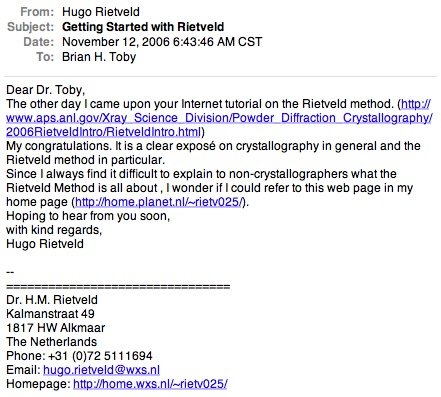
\includegraphics[width=0.75\linewidth]{figures/Hugo.jpg}
    \caption{Brian showing off: Fan mail from Hugo. Note that 20 years later, none of the links in the e-mail still work.}
    \label{fig:Hugo}
\end{figure}

\section{Le Bail Fitting}\label{ref:LeBail}\index{Le Bail fitting}

(more work needed: \ref{needs more work})


\section{Pawley Fitting}\label{ref:Pawley}\index{Pawley fitting}

\section{Fourier Maps}\label{ref:Fourier}

\section{Charge Flipping}